\documentclass[10pt,a4paper]{article}
\usepackage[margin=22mm]{geometry}
\usepackage[T1]{fontenc}
\usepackage{lmodern,microtype,amsmath,amssymb,booktabs,graphicx}
\usepackage[hidelinks]{hyperref}
\usepackage{caption}
\captionsetup{font=small,labelfont=bf}
\setlength{\parskip}{3pt}
\setlength{\parindent}{1em}
\setlength{\emergencystretch}{1em}
\newcommand{\BatchMean}{5.551\times10^{-16}}
\newcommand{\BatchCov}{1.249\times10^{-16}}
\newcommand{\BatchNll}{8.882\times10^{-16}}
\newcommand{\QuadError}{1.388\times10^{-17}}
\newcommand{\StationaryError}{2.220\times10^{-16}}
\newcommand{\FilterSd}{0.07077}
\newcommand{\SmoothSd}{0.06111}
\newcommand{\Reduction}{25.44}
\newcommand{\FilterNees}{1.949}
\newcommand{\SmoothNees}{1.912}
\newcommand{\FilterCoverage}{96.88}
\newcommand{\SmoothCoverage}{97.66}
\newcommand{\NeesLow}{1.762}
\newcommand{\NeesHigh}{2.252}
\newcommand{\EulerRows}{16 & 0.062500 & 2.57861 & 0.40797 \\
32 & 0.031250 & 0.73195 & 0.14898 \\
64 & 0.015625 & 0.33249 & 0.06210 \\
128 & 0.007812 & 0.16029 & 0.02834 \\
256 & 0.003906 & 0.07867 & 0.01354 \\}

\title{GapSmooth: exact stochastic vibration inference\\across a sensor outage}
\author{}
\date{}
\begin{document}
\maketitle
\vspace{-1.6em}
\begin{abstract}
Missing displacement measurements create uncertainty about both displacement
and velocity in vibrating systems. This reproducible software study asks how
much future measurements reduce uncertainty inside a known outage under a
linear Gaussian model. An exactly sampled stochastic oscillator is combined
with Joseph-form Kalman filtering and Rauch--Tung--Striebel smoothing. Independent
batch conditioning and covariance quadrature verify different parts of the
calculation. In the recorded synthetic experiment, smoothing reduces midpoint
displacement variance by \Reduction\%, while retaining nonzero uncertainty.
An ensemble of 256 independent trajectories checks fixed-time calibration.
Euler refinement separates time-discretization error from discrete inference
error. Results establish consistency with the stated model, not physical validity.
\end{abstract}

\section{Question, model and assumptions}
A sensor outage does not freeze a structure: unobserved forcing continues to
perturb its state. Future measurements can constrain an earlier trajectory,
but cannot remove all uncertainty. The research question is therefore a
conditional one: for specified dynamics, noise and sampling, how much smaller
is the offline posterior variance than the causal filtering variance?
The work connects state-space and Kalman-estimation concepts identified in the
local DTU advanced time-series lectures with a mechanical vibration mode.
No private course material, solutions or data are redistributed.

Let $z=(x,v)^T$, with displacement $x$ in metres and velocity $v$ in metres per
second. A mass-normalized damped mode obeys the It\^o SDE
\begin{equation}
 dz=A z\,dt+L\,dW,\qquad
 A=\begin{bmatrix}0&1\\-\omega^2&-2\zeta\omega\end{bmatrix},\quad
 D=LL^T=\begin{bmatrix}0&0\\0&q\end{bmatrix}.
 \label{eq:model}
\end{equation}
Here $\omega>0$, $\zeta>0$ and $q\geq0$; $q$ has units
$\mathrm{m}^2\mathrm{s}^{-3}$. Observations are $y_k=Hz_k+\epsilon_k$,
$H=[1,0]$, with independent $\epsilon_k\sim\mathcal N(0,R)$ and $R>0$.
The initial Gaussian state, process noise and sensor noise are mutually
independent. Parameters and the missing-data schedule are known. The model
excludes nonlinear restoring forces, colored forcing and parameter uncertainty.
The white-noise forcing is an idealization, not a measured load.

\section{Numerical method and implementation}
Linear SDE transition moments are available without time-stepping truncation
\cite{sde}. For interval $h$,
\begin{equation}
 F(h)=e^{Ah},\qquad Q(h)=\int_0^h e^{As}D e^{A^Ts}\,ds,\qquad
 z_{k+1}\mid z_k\sim\mathcal N(Fz_k,Q).
 \label{eq:transition}
\end{equation}
The implementation exponentiates $h[\begin{smallmatrix}A&D\\0&-A^T\end{smallmatrix}]$;
its upper blocks are $F,B$, and $Q=BF^T$. Before exponentiation the interval is
scaled until $h\|A\|_\infty\leq1$, then reconstructed by repeated composition
$F\leftarrow F^2$, $Q\leftarrow FQF^T+Q$ using the previous $F,Q$.
This avoids large unstable auxiliary blocks for long intervals. Matrices are
symmetrized to remove antisymmetric roundoff; eigenvalues are not clipped.

For each time, predict $m^-=Fm$, $P^-=FPF^T+Q$. If a measurement exists,
$S=HP^-H^T+R$, $K=P^-H^T/S$, and
\begin{equation}
 m=m^-+K(y-Hm^-),\qquad
 P=(I-KH)P^-(I-KH)^T+KRK^T.
\end{equation}
Missing observations skip the update. The observed-data negative log likelihood
sums $[\log(2\pi S)+(y-Hm^-)^2/S]/2$ over available observations only.
The backward smoother uses $G_k=P_kF_k^T(P^-_{k+1})^{-1}$,
$m_k^s=m_k+G_k(m_{k+1}^s-m^-_{k+1})$ and
$P_k^s=P_k+G_k(P_{k+1}^s-P^-_{k+1})G_k^T$ \cite{bfs}.
Linear solves compute gains; explicit matrix inversion is avoided.

\clearpage
\section{Reproducible experiment}
The original Python package separates dynamics, recursive inference, a dense
reference and experiment generation. NumPy and SciPy supply compiled small-matrix
operations; a separate C++ binding is unnecessary for this two-state experiment.
The recursive algorithm has linear work and storage in record length for fixed
state dimension. The dense reference constructs the full joint state Gaussian
and conditions all observed displacements in one solve; it is limited to 256
times because of quadratic storage and cubic solve cost.

The experiment uses $\omega=2\pi\ \mathrm{rad/s}$, $\zeta=0.08$, $q=0.6$,
$R=0.02^2\ \mathrm{m}^2$ and $t_k=k/16$ for $k=0,\ldots,128$.
Measurements at $3\leq t_k\leq5$ s are removed (33 samples). The zero-mean
initial state has the analytical stationary covariance
\begin{equation}
 P_\infty=\operatorname{diag}\left(
 \frac{q}{4\zeta\omega^3},\frac{q}{4\zeta\omega}\right).
 \label{eq:stationary}
\end{equation}
The prior is at the first supplied time, before its observation. Synthetic truth
is generated from exact transition moments; seed 2718 gives Fig.~\ref{fig:outage}.
Filtering is causal; smoothing conditions on the entire record through 8 s.
The sampling interval differs from any hidden integration step: there is none.

\begin{figure}[ht]
 \centering
 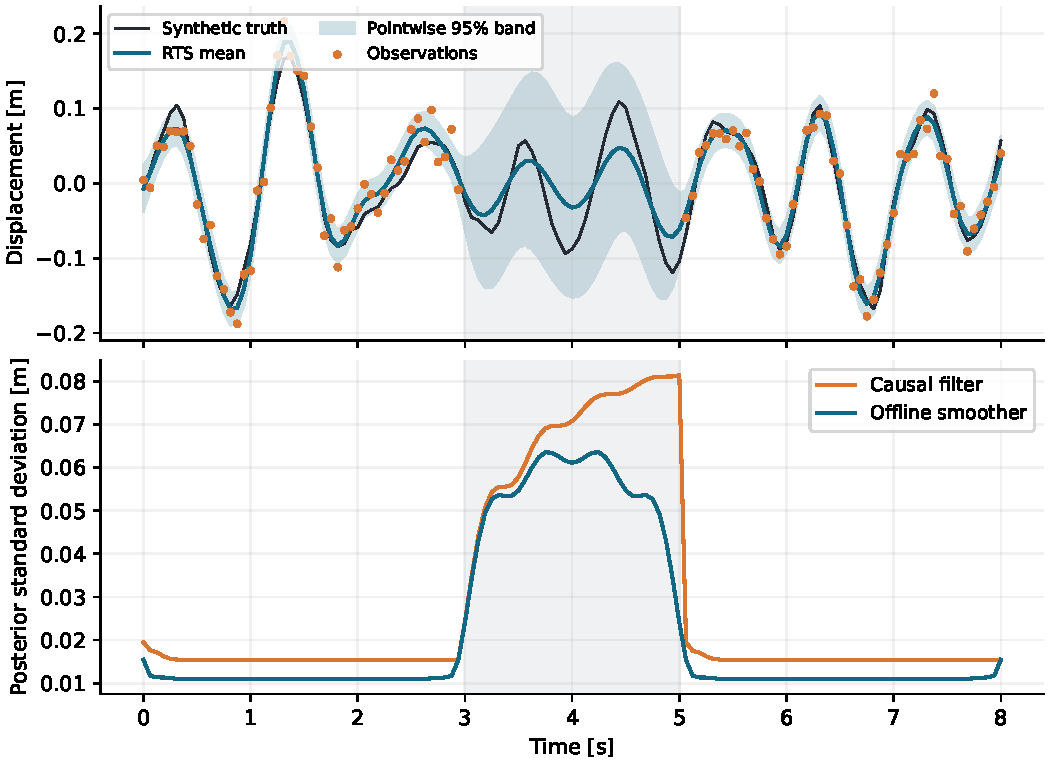
\includegraphics[width=0.92\linewidth]{../examples/results/outage.pdf}
 \caption{Original synthetic trajectory and uncertainty. Shading marks the
 missing-measurement interval. The blue band is a pointwise 95\% smoothed
 displacement interval, not a simultaneous trajectory band. Future observations
 reduce uncertainty near both sides of the gap; the middle remains uncertain.}
 \label{fig:outage}
\end{figure}

At $t=4$ s the filtered displacement standard deviation is $\FilterSd$ m and
the smoothed value is $\SmoothSd$ m, a variance reduction of \Reduction\%.
Because this is a linear model with fixed noise, both posterior covariance
sequences depend on the observation schedule but not the observed values.
This reduction is not a claim that smoothing improves every realized squared error.

An ensemble of 256 independent trajectories uses seeds 10000--10255 and the
same prior, dynamics and outage. Only $t=4$ s is used for calibration statistics:
temporal samples are not counted as independent trials. For state error $e$,
the normalized estimation error squared is $e^TP^{-1}e$ (NEES). Its expected
value is two; the ensemble mean has a 95\% model-consistency interval
$[\NeesLow,\NeesHigh]$ from $\chi^2_{512}/256$. Observed means are
\FilterNees\ (filter) and \SmoothNees\ (smoother). Displacement coverage of
pointwise 95\% intervals is \FilterCoverage\% and \SmoothCoverage\%, respectively.
These finite-sample diagnostics are correlated between methods and do not prove
calibration outside the generating model.

\clearpage
\section{Verification and separation of errors}
\textbf{Discrete inference.} On a nine-time irregular grid with four missing
samples, the maximum differences from dense Gaussian conditioning are
$\BatchMean$ for state means and $\BatchCov$ for marginal covariances;
the likelihood difference is $\BatchNll$. Prefix-conditioned batch estimates
also verify causal filtering. This checks the recursion but shares transition
moments, so it cannot alone verify Eq.~\eqref{eq:transition}.

\textbf{Continuum moments.} Independent adaptive quadrature of the covariance
integral at $h=0.3$ s differs by at most $\QuadError$; the stationary identity
$FP_\infty F^T+Q=P_\infty$ differs by $\StationaryError$.
Additional tests cover semigroup composition, $h=0$, tiny and long intervals,
zero process intensity, absent observations, input errors and covariance reduction.
Exact sampled moments have floating-point error, but no time-step truncation
for Eq.~\eqref{eq:model}. No continuum sample-path accuracy is claimed.

For contrast, forward Euler uses $F_E=I+hA$ and $Q_E=hD$. Composing these
over one second yields Table~\ref{tab:euler}. Errors use Frobenius norms with
coordinates scaled by 1 m, 1 m/s and 1 s; their values depend on this scaling.
This compares deterministic moments, not different random trajectories.

\begin{table}[ht]
 \centering
 \caption{Recorded Euler errors against exact one-second transition moments.}
 \label{tab:euler}
 \begin{tabular}{rrrr}
 \toprule
 Steps & $h$ [s] & $\|F_E^{\rm composed}-F(1)\|_F$ & $\|Q_E^{\rm composed}-Q(1)\|_F$\\
 \midrule
 \EulerRows
 \bottomrule
 \end{tabular}
\end{table}
The recorded moment errors decrease as the Euler step is refined. Coarse steps
can be unstable; this is not an unconditional stability or asymptotic-order claim.

\section{Discussion, limitations and conclusion}
The measured variance reduction quantifies the benefit of future information
for one known model and schedule. It does not eliminate uncertainty caused by
unobserved forcing. Discrete posterior agreement, continuum moment verification,
and model-based coverage address distinct questions; none validates a physical
structure. Experimental data, uncertain parameters, nonlinear mechanics and
model mismatch remain outside scope. Covariance-form filtering can lose accuracy
in extreme conditioning; a square-root implementation would require separate
verification. The work claims no new filtering theory or peer review.

Reproduce with \texttt{pip install -e ".[dev]"}, then
\texttt{gapsmooth --output reproduced}. Recorded metrics, CSV trace and figures
are versioned. Tests, lint, package builds and sample reproduction are automated.
Run \texttt{python paper/build.py --engine pdflatex} to generate data-bound
numbers, compile, check references/layout warnings and enforce the five-page
limit. A hash manifest links the PDF to code and numerical inputs; page rendering
supports a separate human-style visual inspection.

\begin{thebibliography}{9}
\bibitem{sde} S.~S\"arkk\"a and A.~Solin. \emph{Applied Stochastic Differential
Equations}. Cambridge University Press, 2019. Chapters 6 and 10.
\href{https://users.aalto.fi/~asolin/sde-book/sde-book.pdf}{Author-hosted text}.
\bibitem{bfs} S.~S\"arkk\"a and L.~Svensson. \emph{Bayesian Filtering and Smoothing}.
2nd ed., Cambridge University Press, 2023.
\href{https://users.aalto.fi/~ssarkka/pub/bfs_book_2023_online.pdf}{Author-hosted text}.
\end{thebibliography}
\end{document}
